\documentclass[11pt,letterpaper,oneside]{article}
\renewcommand{\abstractname}{Executive Summary}
\usepackage{graphicx}
\begin{document}
\begin{abstract}
Defining neighborhoods based on residents perceptions requires an
unfeasibly large sample for survey research. Real estate information
that identifies neighborhoods is plentiful, but certainly biased. I
propose to compare survey responses about neighborhood perception with
data from real estate listings to characterize the bias and evaluate
whether listing data may be an acceptable measure of residents
perceptions of neighborhoods.
\end{abstract}

In the long history of the ecological effects of neighborhood, we have
faced the perennial problem of how to practically define the
neighborhood as an object of study. Since we think about the
neighborhood as an area defined by how people interact with it and
within it, we have often been tempted to let people define
neighborhoods for us.

Unfortunately, when we ask people to define their neighborhoods we run
into a robust social fact. People have a very hard time drawing the
boundaries of their neighborhood, and if we can elicit two definitions
of neighborhood areas, they are are almost certain to disagree.

Typically when faced with such variation, we respond by averaging
responses together to estimate the central tendency. However, in the
case of neighborhoods, we would need a very large sample in order to
get a stable estimate given that the size of some named neighborhoods
are quite small.

I propose that we may be able to measure residents’ perceptions
indirectly, by looking at what neighborhood real estate listings claim
a location is in. The obvious virtue of such data are their volume,
and if they are not too inaccurate, they could allow for a very high
resolution cognitive map of a city.

For the past year, I have download Chicago Craigslist apartment,
rental, sublet and roommate listings, nightly. When a persons posts a
listing, they have the option of putting in an address or
intersection. This allows me to associate latitude and longitude with
a posting. They also have the option of entering, in free text, the
“Specific location” of the posting.  With these data, I can estimate
how likely that a listing will say that a location is in a
neighborhood (Figure 1).

We should expect these data to be biased, but how much? If these data
should prove usable, then we would have a powerful and inexpensive way
of getting at how people divide up their cities.

In order to evaluate these data, we must compare it to data that we
expect to be generally unbiased. In the 1994 Project on Human
Development in Chicago Neighborhoods Community Survey, the second and
third questions asked the respondents the name of the neighborhood and
to define its boundaries.

I request access to the responses to these two questions as well as
information about the location of where the interview took place. With
these data, I can begin to characterize the nature and extent of bias
of the real estate listing data. While we would prefer to use data
that was not 20 years old, I expect that it should be useful for these
purposes since neighborhoods do not seem to change all that quickly.

\begin{figure}
\centering
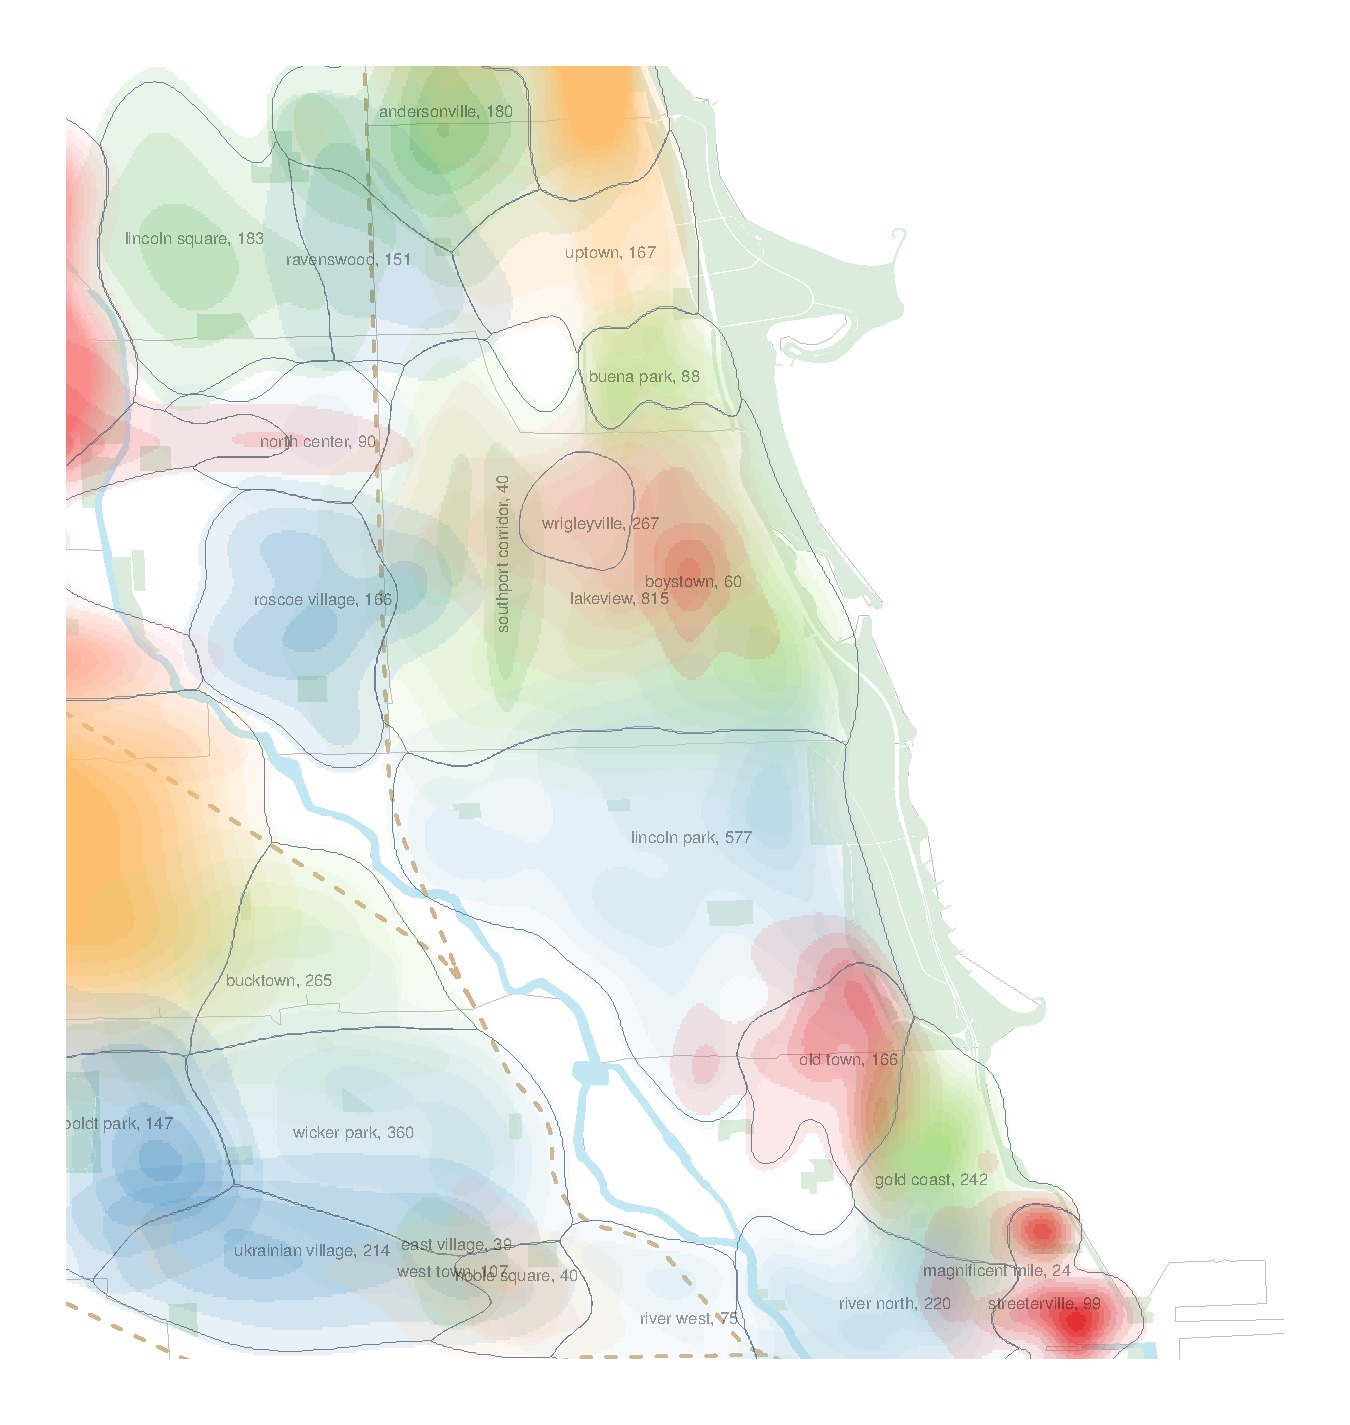
\includegraphics[width=\textwidth]{../presentations/presentation_images/ksplot.pdf}
\caption{Estimate of a Craigslist Listing Nominating a Neighborhood}
\end{figure}
\end{document}